%\def\demsode{1}
%\begin{name}
%	{Biên soạn: Vu Long}
%	{ĐỀ CHUYÊN TRẦN PHÚ HẢI PHÒNG LẦN 1}
%\end{name}
\section{Chuyên Trần Phú -- Hải Phòng, Lần 1 25--26}
 
\Opensolutionfile{ansbook}[ans/ansb\currfilebase]

\caulc
\Opensolutionfile{ans}[ans/ans\currfilebase-Phan-I]

\begin{ex}%[2D1H5-1]
	\immini[thm]
	{Đồ thị của hàm số nào dưới đây có dạng như đường cong trong hình vẽ?
	\choice
	{$y=\dfrac{2x-1}{2x+1}$}
	{\True $y=\dfrac{x+1}{x-1}$}
	{$y=\dfrac{2x+1}{2x-1}$}
	{$y=\dfrac{2x+1}{x-1}$}}
	{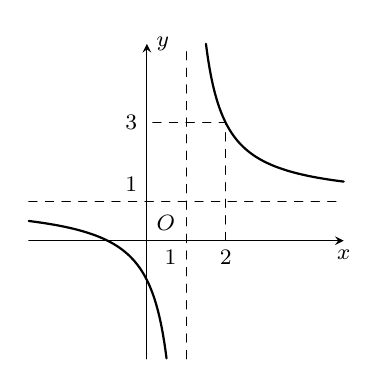
\begin{tikzpicture}[scale=0.5, font=\footnotesize, line join=round, line cap=round, >=stealth]
		\draw[->] (-3,0) -- (5,0) node[below] {$x$};
		\draw[->] (0,-3) -- (0,5) node[right] {$y$};
		\draw (0,0) node[above right] {$O$};
		\draw[dashed] (1,-3)--(1,5);
		\draw[dashed] (-3,1)--(5,1);
		\draw[dashed] (2,0)--(2,3)--(0,3);
		\draw (1,0) node[below left] {$1$};
		\draw (2,0) node[below] {$2$};
		\draw (0,1) node[above left] {$1$};
		\draw (0,3) node[left] {$3$};
		%\clip (-4,-4) rectangle (5,5);
		\draw[thick, smooth, samples=100, domain=1.5:5] plot(\x, {(\x+1)/(\x-1)});
		\draw[thick, smooth, samples=100, domain=-3:0.5] plot(\x, {(\x+1)/(\x-1)});
	\end{tikzpicture}}
	\loigiai{
		Dựa vào đồ thị ta thấy
		\begin{itemize}
			\item Đồ thị hàm số có tiệm cận đứng là $x=1$.
			\item Đồ thị hàm số có tiệm cận ngang là $y=1$.
			\item Đồ thị đi qua điểm $(2;3)$ và $(0;-1)$.
		\end{itemize}
		Đồ thị hàm số $y=\dfrac{x+1}{x-1}$ có tiệm cận đứng $x=1$; tiệm cận ngang $y=1$ và đi qua điểm $(2;3)$.\\
		Vậy đồ thị trên là đồ thị của hàm số $y=\dfrac{x+1}{x-1}$.
	}
\end{ex}

\begin{ex}%[2H2H1-2]
	\immini[thm]
	{Cho hình hộp $ABCD.A'B'C'D'$ tâm $O$. Gọi $I$, $I'$ lần lượt là tâm của hình bình hành $ABCD$, $A'B'C'D'$ (hình vẽ). Khẳng định nào sau đây sai?
	\choice
	{$\overrightarrow{AC'}=\overrightarrow{AB}+\overrightarrow{AD}+\overrightarrow{AA'}$}
	{$\overrightarrow{OI}+\overrightarrow{OI'}=\overrightarrow{0}$}
	{\True $\overrightarrow{AB}+\overrightarrow{AA'}=\overrightarrow{AD}+\overrightarrow{DD'}$}
	{$\overrightarrow{AB}+\overrightarrow{BC}+\overrightarrow{CC'}=\overrightarrow{AC'}$}}
	{\begin{tikzpicture}[scale=0.8, line join=round, line cap=round, >=stealth]
		% Định nghĩa các điểm bằng tọa độ thủ công để không dùng tkz-euclide
		\coordinate (D) at (0,0);
		\coordinate (C) at (4.5,0);
		\coordinate (A) at (1.25,1.5);
		\coordinate (B) at ($(A) + (C) - (D)$);		
		\coordinate (D') at (0,4);
		\coordinate (C') at ($(C)+(D')-(D)$);
		\coordinate (A') at ($(A)+(D')-(D)$);
		\coordinate (B') at ($(B)+(D')-(D)$);
		\coordinate (I) at ($(A)!0.5!(C)$);
		\coordinate (I') at ($(A')!0.5!(C')$);
		\coordinate (O) at ($(I)!0.5!(I')$);
		\draw (D)--(C)--(B)--(B')--(C')--(D')--(D);
		\draw (C)--(C');
		\draw (B')--(A')--(D');
		\draw[dashed] (A)--(B) (A)--(D) (A)--(A');
		\draw[dashed] (A)--(C) (B)--(D);
		\draw (A')--(C') (B')--(D');
		\draw[dashed] (I)--(I');
		\draw[dashed] (A)--(C') (B)--(D') (C)--(A') (D)--(B');
		\foreach \p in {A,B,C,D,A',B',C',D',I,I',O} \fill (\p) circle (1.5pt);
		\node[left] at (A) {$A$};
		\node[right] at (B) {$B$};
		\node[right] at (C) {$C$};
		\node[left] at (D) {$D$};
		\node[left] at (A') {$A'$};
		\node[right] at (B') {$B'$};
		\node[right] at (C') {$C'$};
		\node[left] at (D') {$D'$};
		\node[below] at (I) {$I$};
		\node[above] at (I') {$I'$};
		\node[right] at (O) {$O$};
	\end{tikzpicture}}
	\loigiai{
		Ta có
		\begin{itemize}
			\item $\overrightarrow{AC'}=\overrightarrow{AB}+\overrightarrow{AD}+\overrightarrow{AA'}$ đúng theo quy tắc hình hộp.
			\item $\overrightarrow{OI}+\overrightarrow{OI'}=\overrightarrow{0}$ đúng vì $O$ là trung điểm của $II'$.
			\item $\overrightarrow{AB}+\overrightarrow{BC}+\overrightarrow{CC'}=\overrightarrow{AC'}$ đúng theo quy tắc cộng vectơ.
		\end{itemize}
		Xét khẳng định $\overrightarrow{AB}+\overrightarrow{AA'}=\overrightarrow{AD}+\overrightarrow{DD'}$.\\
		Vế trái $\overrightarrow{AB}+\overrightarrow{AA'}=\overrightarrow{AB'}$.\\
		Vế phải $\overrightarrow{AD}+\overrightarrow{DD'}=\overrightarrow{AD'}$.\\
		Vì $\overrightarrow{AB'} \ne \overrightarrow{AD'}$ nên khẳng định này sai.
	}
\end{ex}

\begin{ex}%[2D3H2-2]
	Mỗi ngày bác Lan đều đi bộ để rèn luyện sức khoẻ. Quãng đường đi bộ mỗi ngày (đơn vị: km) của bác Lan trong $20$ ngày được thống kê lại ở bảng sau:
	\begin{center}
		\begin{tabular}{|c|c|c|c|c|c|}
			\hline
			Quãng đường (km) & $[2{,}7;3{,}0)$ & $[3{,}0;3{,}3)$ & $[3{,}3;3{,}6)$ & $[3{,}6;3{,}9)$ & $[3{,}9;4{,}2)$\\
			\hline
			Số ngày & $3$ & $6$ & $5$ & $4$ & $2$\\
			\hline
		\end{tabular}
	\end{center}
	Độ lệch chuẩn của mẫu số liệu ghép nhóm có giá trị gần nhất với giá trị nào dưới đây?
	\choice
	{$3{,}41$}
	{\True $0{,}36$}
	{$0{,}13$}
	{$0{,}017$}
	\loigiai{
		Bảng giá trị đại diện
		\begin{center}
			\begin{tabular}{|c|c|c|c|c|c|}
				\hline
				Quãng đường & $[2{,}7; 3{,}0)$ & $[3{,}0; 3{,}3)$ & $[3{,}3; 3{,}6)$ & $[3{,}6; 3{,}9)$ & $[3{,}9; 4{,}2)$\\
				\hline
				Giá trị đại diện ($x_i$) & $2{,}85$ & $3{,}15$ & $3{,}45$ & $3{,}75$ & $4{,}05$\\
				\hline
				Số ngày ($n_i$) & $3$ & $6$ & $5$ & $4$ & $2$\\
				\hline
			\end{tabular}
		\end{center}
		Cỡ mẫu $n = 20$.\\
		Giá trị trung bình của mẫu số liệu ghép nhóm là $\overline{x}=\dfrac{2{,}85 \cdot 3 + 3{,}15 \cdot 6 + 3{,}45 \cdot 5 + 3{,}75 \cdot 4 + 4{,}05 \cdot 2}{20}=3{,}39$.\\
		Phương sai $s^2 = \dfrac{1}{20}\left(3 \cdot 2{,}85^{2} + 6 \cdot 3{,}15^{2} + 5 \cdot 3{,}45^{2} + 4 \cdot 3{,}75^{2} + 2 \cdot 4{,}05^{2}\right) - 3{,}39^{2} \approx 0{,}1314$.\\
		Độ lệch chuẩn của mẫu số liệu ghép nhóm $s = \sqrt{0{,}1314} \approx 0{,}36$.
	}
\end{ex}

\begin{ex}%[2D1N1-2]
	\immini[thm]
	{Cho hàm số $y=f(x)$ liên tục trên $\mathbb{R}$ và có đồ thị là đường cong trong hình dưới đây. Hàm số đã cho đồng biến trên khoảng nào dưới đây?
	\choice
	{\True $(0;1)$}
	{$(-1;1)$}
	{$(-\infty;1)$}
	{$(0;+\infty)$}}
	{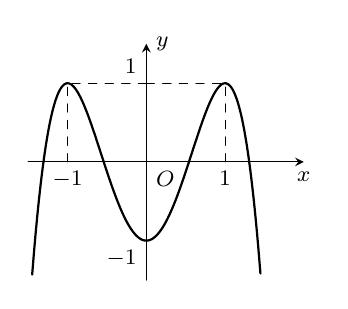
\begin{tikzpicture}[scale=1, font=\footnotesize, line join=round, line cap=round, >=stealth]
		\draw[->] (-1.5,0) -- (2,0) node[below] {$x$};
		\draw[->] (0,-1.5) -- (0,1.5) node[right] {$y$};
		\draw (0,0) node[below right] {$O$};
		\draw[dashed] (-1,0) node[below]{$-1$} -- (-1,1) -- (0,1);
		\draw[dashed] (1,0) node[below]{$1$} -- (1,1) -- (0,1) node[above left]{$1$};
		\draw (0,-1) node[below left]{$-1$};
		\draw[thick, smooth, samples=100, domain=-1.45:1.45] plot(\x, {-2*(\x)^4 + 4*(\x)^2 - 1});
	\end{tikzpicture}}
	\loigiai{
		Quan sát đồ thị, ta thấy đồ thị hàm số đi lên trong khoảng $(0;1)$.\\
		Vậy hàm số đã cho đồng biến trên khoảng $(0;1)$.
	}
\end{ex}

\begin{ex}%[2H2N2-3]
	Trong không gian $Oxyz$, cho hai vectơ $\overrightarrow{a}=(2;2;3)$, $\overrightarrow{b}=\overrightarrow{j}-2\overrightarrow{k}$. Tính tọa độ vectơ $\overrightarrow{u}=\overrightarrow{a}+\overrightarrow{b}$.
	\choice
	{$(3;2;1)$}
	{\True $(2;3;1)$}
	{$(2;1;5)$}
	{$(3;0;3)$}
	\loigiai{
		Ta có $\overrightarrow{a}=(2;2;3)$, $\overrightarrow{b}=\overrightarrow{j}-2\overrightarrow{k} \Rightarrow \overrightarrow{b}=(0;1;-2)$.\\
		Tọa độ vectơ $\overrightarrow{u}=\overrightarrow{a}+\overrightarrow{b}=(2+0;2+1;3-2)=(2;3;1)$.
	}
\end{ex}

\begin{ex}%[1D6H4-4]
	Tập nghiệm của bất phương trình $\left(2-\sqrt{3}\right)^{x-1} \le \left(2+\sqrt{3}\right)^{-x^{2}+x+9}$ là
	\choice
	{$(-\infty;-4] \cup [2;+\infty)$}
	{$(-\infty;-2] \cup [4;+\infty)$}
	{\True $[-2;4]$}
	{$[-4;2]$}
	\loigiai{
		Ta có $\left(2-\sqrt{3}\right)\left(2+\sqrt{3}\right)=1 \Rightarrow 2-\sqrt{3}=\left(2+\sqrt{3}\right)^{-1}$.\\
		Bất phương trình trở thành $\left(2+\sqrt{3}\right)^{-(x-1)} \le \left(2+\sqrt{3}\right)^{-x^{2}+x+9}$.\\
		Vì cơ số $2+\sqrt{3} > 1$ nên bất phương trình tương đương với
		\[-(x-1) \le -x^{2}+x+9 \Leftrightarrow x^{2}-2x-8 \le 0 \Leftrightarrow -2 \le x \le 4.\]
		Vậy tập nghiệm của bất phương trình là $[-2;4]$.
	}
\end{ex}

\begin{ex}%[1D5H2-3]
	Kết quả bài kiểm tra môn Toán cuối học kỳ I của học sinh khối $12$ một trường THPT được ghi lại ở bảng sau:
	\begin{center}
		\begin{tabular}{|c|c|c|c|c|c|}
			\hline
			Điểm số & $[0;2)$ & $[2;4)$ & $[4;6)$ & $[6;8)$ & $[8;10]$\\
			\hline
			Số học sinh & $24$ & $67$ & $136$ & $167$ & $106$\\
			\hline
		\end{tabular}
	\end{center}
	Dựa vào bảng số liệu trên, giáo viên Toán có thể nhận định $75\%$ học sinh trong khối có điểm kiểm tra Toán cuối học kỳ I từ bao nhiêu trở lên?
	\choice
	{$4{,}0$}
	{$5{,}0$}
	{\True $4{,}5$}
	{$5{,}5$}
	\loigiai{
		Câu hỏi "$75\%$ học sinh có điểm từ bao nhiêu trở lên" tương ứng với việc tìm tứ phân vị thứ nhất $Q_1$ (giá trị mà có $25\%$ số liệu thấp hơn nó và $75\%$ số liệu cao hơn nó).\\
		Ta có tổng số học sinh $n=500 \Rightarrow \dfrac{n}{4}=125$.\\
		Tần số tích lũy của nhóm $[0;2)$ là $24$.\\
		Tần số tích lũy của nhóm $[2;4)$ là $24+67=91 < 125$.\\
		Tần số tích lũy của nhóm $[4;6)$ là $91+136=227 > 125$.\\
		Do đó nhóm chứa tứ phân vị thứ nhất là $[4;6)$.\\
		Áp dụng công thức ta được
		\[Q_1 = 4 + \dfrac{125-91}{136} \cdot (6-4) = 4 + \dfrac{34}{136} \cdot 2 = 4 + 0{,}5 = 4{,}5.\]
		Vậy $75\%$ học sinh có điểm từ $4{,}5$ trở lên.
	}
\end{ex}

\begin{ex}%[2H2H2-4]
	Trong không gian $Oxyz$, cho hai vectơ $\overrightarrow{u}=(1;1;-\sqrt{2})$, $\overrightarrow{v}=(1;0;m)$. Có bao nhiêu giá trị của $m$ để góc giữa hai vectơ $\overrightarrow{u}$ và $\overrightarrow{v}$ bằng $60^{\circ}$?
	\choice
	{$4$}
	{$2$}
	{$0$}
	{\True $1$}
	\loigiai{
		Ta có $|\overrightarrow{u}|=\sqrt{1^2+1^2+\left(-\sqrt{2}\right)^2}=\sqrt{4}=2$.\\
		$|\overrightarrow{v}|=\sqrt{1^2+0^2+m^2}=\sqrt{1+m^2}$.\\
		Tích vô hướng $\overrightarrow{u} \cdot \overrightarrow{v} = 1 \cdot 1 + 1 \cdot 0 + \left(-\sqrt{2}\right) \cdot m = 1 - m\sqrt{2}$.\\
		Theo giả thiết góc giữa hai vectơ bằng $60^{\circ}$ nên
		\allowdisplaybreaks
		\begin{eqnarray*}
			&& \cos\left(\overrightarrow{u},\overrightarrow{v}\right) = \dfrac{\overrightarrow{u} \cdot \overrightarrow{v}}{\left|\overrightarrow{u}\right| \cdot \left|\overrightarrow{v}\right|} = \cos 60^{\circ} = \dfrac{1}{2}\\
			&\Leftrightarrow& \dfrac{1-m\sqrt{2}}{2\sqrt{1+m^2}} = \dfrac{1}{2}\\
			 &\Leftrightarrow& 1-m\sqrt{2} = \sqrt{1+m^2}\\
			&\Leftrightarrow& \heva{& 1-m\sqrt{2} \ge 0\\ &(1-m\sqrt{2})^2 = 1+m^2}\\
			& \Leftrightarrow& \heva{&m \le \dfrac{1}{\sqrt{2}}\\ &1-2m\sqrt{2}+2m^2 = 1+m^2}\\
			&\Leftrightarrow& \heva{& m \le \dfrac{\sqrt{2}}{2}\\ &m^2-2m\sqrt{2} = 0}\\
			& \Leftrightarrow& \heva{& m \le \dfrac{\sqrt{2}}{2}\\ &\hoac{&m=0\\ &m=2\sqrt{2}.} }
		\end{eqnarray*}
		Đối chiếu điều kiện, ta thấy chỉ có $m=0$ thỏa mãn.\\
		Vậy có $1$ giá trị của $m$ thỏa mãn.
	}
\end{ex}

\begin{ex}%[2D1H2-1]
	Số điểm cực tiểu của đồ thị hàm số $y=\dfrac{1}{5}x^5-\dfrac{3}{4}x^4+\dfrac{2}{3}x^3+\dfrac{1}{2}$ là
	\choice
	{$0$}
	{$3$}
	{$2$}
	{\True $1$}
	\loigiai{
		Tập xác định $\mathscr{D}=\mathbb{R}$.\\
		Ta có $y' = x^4 - 3x^3 + 2x^2 = x^2(x^2 - 3x + 2)$.\\
		$y' = 0 \Leftrightarrow \hoac{&x=0\,\,\text{nghiệm kép}\\ &x=1\\ &x=2.}$\\
		Bảng biến thiên
		\begin{center}
			
\begin{tikzpicture}
				\tkzTabInit[lgt=1.2,espcl=2.5]
				{$x$ /1, $y'$ /1, $y$ /2}
				{$-\infty$, $0$, $1$, $2$, $+\infty$}
				\tkzTabLine{,+,0,+,0,-,0,+,}
				\tkzTabVar{-/ $-\infty$, R/, +/ $y(1)$, -/ $y(2)$, +/ $+\infty$}
			\end{tikzpicture}
		\end{center}
		Từ bảng biến thiên, ta thấy đồ thị hàm số có $1$ điểm cực tiểu tại $x=2$.
	}
\end{ex}

\begin{ex}%[2H2N2-2]
	Trong không gian $Oxyz$, cho vectơ $\overrightarrow{MN}=(2;-1;5)$ và điểm $N(0;3;-1)$. Điểm $M$ có tọa độ là
	\choice
	{$(-2;-2;-4)$}
	{\True $(-2;4;-6)$}
	{$(2;-4;6)$}
	{$(2;2;4)$}
	\loigiai{
		Gọi $M(x;y;z)$.\\
		Ta có $\overrightarrow{MN} = (0-x; 3-y; -1-z)$.\\
		Theo đề bài $\overrightarrow{MN}=(2;-1;5)$ nên ta có hệ phương trình: $\begin{cases} 0-x=2\\ 3-y=-1\\ -1-z=5 \end{cases} \Leftrightarrow \begin{cases} x=-2\\ y=4\\ z=-6. \end{cases}$\\
		Vậy tọa độ điểm $M$ là $(-2;4;-6)$.
	}
\end{ex}

\begin{ex}%[1D2H2-6]
	Cho cấp số cộng $(u_n)$ có $u_1=\dfrac{1}{4}$ và $d=-\dfrac{1}{4}$. Gọi $S_5$ là tổng $5$ số hạng đầu tiên của cấp số cộng đã cho. Mệnh đề nào sau đây đúng?
	\choice
	{$S_5=\dfrac{5}{4}$}
	{\True $S_5=-\dfrac{5}{4}$}
	{$S_5=\dfrac{4}{5}$}
	{$S_5=-\dfrac{4}{5}$}
	\loigiai{
		Tổng $5$ số hạng đầu tiên của cấp số cộng là
		\[S_5 = \dfrac{5(2u_1 + 4d)}{2} = \dfrac{5\left[2 \cdot \dfrac{1}{4} + 4 \cdot \left(-\dfrac{1}{4}\right)\right]}{2} = \dfrac{5\left(\dfrac{1}{2} - 1\right)}{2} = \dfrac{5 \cdot \left(-\dfrac{1}{2}\right)}{2} = -\dfrac{5}{4}.\]
	}
\end{ex}

\begin{ex}%[2H2N2-2]
	Cho các điểm $A(1;-2;3)$, $B(-2;1;2)$, $C(3;-1;2)$. Khẳng định nào sau đây đúng?
	\choice
	{Ba điểm $A$, $B$, $C$ thẳng hàng}
	{$BC=8$}
	{\True Trung điểm đoạn thẳng $AB$ có tọa độ là $\left(-\dfrac{1}{2};-\dfrac{1}{2};\dfrac{5}{2}\right)$}
	{Tích vô hướng của hai vectơ $\overrightarrow{AB}$ và $\overrightarrow{AC}$ bằng $6$}
	\loigiai{
		\begin{itemize}
			\item Ta có $\overrightarrow{AB}=(-3;3;-1)$, $\overrightarrow{AC}=(2;1;-1)$. Vì $\dfrac{-3}{2} \ne \dfrac{3}{1}$ nên hai vectơ $\overrightarrow{AB}$ và $\overrightarrow{AC}$ không cùng phương, do đó $A$, $B$, $C$ không thẳng hàng.
			\item Tọa độ trung điểm của đoạn thẳng $AB$ là $\left(\dfrac{1+(-2)}{2}; \dfrac{-2+1}{2}; \dfrac{3+2}{2}\right) = \left(-\dfrac{1}{2}; -\dfrac{1}{2}; \dfrac{5}{2}\right)$. Khẳng định này đúng.
			\item $BC = \sqrt{(3-(-2))^2 + (-1-1)^2 + (2-2)^2} = \sqrt{25+4} = \sqrt{29} \ne 8$.
			\item $\overrightarrow{AB} \cdot \overrightarrow{AC} = -3 \cdot 2 + 3 \cdot 1 + (-1) \cdot (-1) = -6 + 3 + 1 = -2 \ne 6$
		\end{itemize}
	}
\end{ex}

\Closesolutionfile{ans}

\cauds
\Opensolutionfile{ans}[ans/ans\currfilebase-Phan-II]

\begin{ex}%[1D1V4-8]
	Một cây cầu bắc qua sông có dạng cung $OA$ của đồ thị hàm số $y=4{,}8 \sin\dfrac{x}{9}$ và được mô tả trong hệ trục tọa độ với đơn vị trục là mét như hình vẽ. Trục $Ox$ nằm trên mặt nước sông.
	\begin{center}
		\definecolor{darkspringgreen}{rgb}{0.09, 0.45, 0.27}
		\definecolor{lightcornflowerblue}{rgb}{0.6, 0.81, 0.93}
		\definecolor{anti-flashwhite}{rgb}{0.95, 0.95, 0.96}
		\definecolor{ceruleanblue}{rgb}{0.16, 0.32, 0.75}
		\definecolor{arsenic}{rgb}{0.23, 0.27, 0.29}
		\definecolor{alizarin}{rgb}{0.82, 0.1, 0.26}
		\definecolor{airforceblue}{rgb}{0.36, 0.54, 0.66}
		\definecolor{beige}{rgb}{0.96, 0.96, 0.86}
		\definecolor{darkchampagne}{rgb}{0.76, 0.7, 0.5}
		\definecolor{antiquewhite}{rgb}{0.98, 0.92, 0.84}
		\definecolor{aurometalsaurus}{rgb}{0.43, 0.5, 0.5}
		\begin{tikzpicture}[line join=round, line cap=round,scale=0.25,transform shape]
			
			\draw[left color=lightcornflowerblue!90,right color=lightcornflowerblue!90, middle color=white] (-9,-7) rectangle (15,9);
			
			\tikzset{song/.pic={ 
					\draw[fill=darkchampagne!70] (-9,1)--(-9,-7)--(15,-7)--(15,8) 
					..controls +(-160:1) and +(20:.3) ..(5,5.5) 
					..controls +(-160:.3) and +(50:2) ..cycle;
					\draw[fill=darkspringgreen] (15,8) 
					..controls +(-160:1) and +(20:.3) ..(5,5.5)
					..controls +(-160:.3) and +(50:1) ..(-9,1)--(-9,6.5)
					..controls +(30:.3) and +(150:1.5) ..(15,8.5)--cycle;
			}}
			\tikzset{cau/.pic={ 
					\draw[fill=aurometalsaurus] (6,7)..controls +(60:2) and +(100:2) ..(15,3)--(15,4.6)
					..controls +(110:1.2) and +(30:2) ..(6,8)--(5,7.7)--(5.4,6.85)--cycle
					;
					\draw (14,4.35)--(12,8)--(7,7.45)(15,4.3)--(12,8)--(9,7.1);
					\draw[fill=black] (12,8)--(11,6.25)--(11.2,6.18)--cycle;
					\draw[fill=black] (12,8)--(12.1,6.57)--(12,6.63)--cycle;
					\draw (14.5,5.2)--(12,8)--(8.1,8.05);
			}}
			
			\tikzset{xa_lan/.pic={
					\def\X{ 
						(-5.4,-1)--(-5.4,-1.7)--(-5.7,-2.05)
						..controls +(-80:.2) and +(120:.2) ..(-5.3,-3)
						..controls +(-40:.2) and +(150:.2) ..(-4,-3.7)
						..controls +(0:.4) and +(-150:.2) ..(1.2,-3)
						..controls +(30:.7) and +(-130:.6) ..(5.7,1)
						..controls +(50:.1) and +(-50:.1) ..(5.6,1.3)--(5.8,1.8)--(5.4,1.9)--(.5,-1.4)--cycle
						;
					}
					\draw[fill=ceruleanblue] (5.4,1.9)--(5.4,2.29)--(4.7,2.32)--(4.7,1.9);
					\draw[fill=ceruleanblue!90] (5.4,1.9)--(.5,-1.4)--(-5.4,-1)--(2,2.2)--cycle;
					\draw[fill=arsenic] (5.8,1.8)--(5.4,1.9)--(5.4,2.19) ..controls +(-10:.1) and +(50:.5) ..cycle;
					
					\fill[ceruleanblue] \X;
					\draw[black]\X;
					%------------------
					\draw[fill=arsenic] (-5.4,-1)--(-5.4,-1.7)--(-5.75,-1.6)--(-5.75,-1.25);
			}}
			
			\tikzset{vien_trang/.pic={
					\def\T{ 
						(-5.4,-1)--(-5.75,-1.25)
						..controls +(-90:.9) and +(-150:1) ..(1.3,-1.5)--(1.3,-1.9)
						..controls +(30:.3) and +(-130:.3) ..(5.6,1.5)--(5.7,1.8)
						..controls +(50:.3) and +(-10:.5) ..(5.4,2.2)--(5.4,2.3)
						..controls +(-15:.8) and +(70:.8) ..(5.7,1.45)--(5.7,1.3)
						..controls +(-140:1) and +(30:1) ..(1.3,-2.2)
						..controls +(-160:1) and +(-30:1.2) ..(-5.8,-2)
						..controls +(150:.3) and +(-160:.3) ..(-5.75,-1.25)
						;
					}
					\fill[anti-flashwhite] \T;
					\draw[black]\T;
			}}
			
			\tikzset{container_D/.pic={
					\def\C1{ 
						(-.8,-1.15)--(.4,-1.25)--(1.9,-.3)--(1.9,.9)--(.9,.94)--(-.8,.15)--cycle
						;
					}
					\fill[alizarin] \C1;
					\draw[black]\C1;
					\draw (1.9,.9)--(.35,.1)--(-.8,.15) (.35,.1)--(.4,-1.25);
			}}
			
			\tikzset{container_X/.pic={
					\def\C2{ 
						(-.8,-1.15)--(.4,-1.25)--(1.9,-.3)--(1.9,.9)--(.9,.94)--(-.8,.15)--cycle
						;
					}
					\fill[airforceblue] \C2;
					\draw[black]\C2;
					\draw (1.9,.9)--(.35,.1)--(-.8,.15) (.35,.1)--(.4,-1.25);
			}}
			
			\tikzset{container_trang/.pic={
					\def\C3{ 
						(-.8,-1.15)--(.4,-1.25)--(1.9,-.3)--(1.9,.9)--(.9,.94)--(-.8,.15)--cycle
						;
					}
					\fill[beige] \C3;
					\draw[black]\C3;
					\draw (1.9,.9)--(.35,.1)--(-.8,.15) (.35,.1)--(.4,-1.25);
			}}
			
			\tikzset{lai/.pic={
					\draw[fill=anti-flashwhite] (-2.1,-2)--(-2.1,-.5)--(-1.45,-.3)--(-1.45,-2)--cycle;
					\draw[fill=anti-flashwhite] (-4.6,-.5)--(-4.6,-2)--(-2.1,-2)--(-2.1,-.5)--cycle;
					\draw[fill=ceruleanblue] (-4.2,-1)--(-2.6,-1.1)--(-2.6,-1.3)--(-4.2,-1.2)--cycle;
					\def\L{ 
						(-4,-.2)
						..controls +(-170:.4) and +(30:.2) ..(-5.1,-.6)
						..controls +(-10:.4) and +(-170:.2) ..(-2,-.75)
						..controls +(30:.4) and +(-150:.2) ..(-1.3,-.4)--(-1.3,-.3)
						..controls +(160:.4) and +(-10:.2) ..cycle
						;
					}
					
					\fill[ceruleanblue] \L;
					\draw[black]\L;
			}}
			
			\tikzset{phao/.pic={
					\fill[arsenic,xscale=.8,rotate=5](3,-1.6) circle (.4cm);
					\fill[white,xscale=.8,rotate=5](3,-1.6) circle (.2cm);
			}}
			
			\tikzset{co/.pic={
					\draw [arsenic,xscale=.8,rotate=5]
					(1,8) ..controls +(60:.4) and +(100:.2) ..(2,8)
					..controls +(60:.4) and +(100:.2) ..(2.8,8);
			}}
			
			\path
			(0,0)pic[scale=1]{song}
			(0,0)pic[scale=1]{xa_lan}
			(3.2,1.8)pic[scale=.8]{container_X}
			(2.5,.9)pic[scale=.5]{container_D}
			(1.72,.38)pic[scale=.5]{container_X} 
			
			(1,2.4)pic[scale=1]{container_trang}
			(1.8,2.4)pic[scale=1]{container_trang}
			(-.5,1.5)pic[scale=1]{container_trang}
			(.95,1.3)pic[scale=1]{container_trang}
			(-3.5,1.3)pic[scale=1]{container_trang}
			(-2.8,1.15)pic[scale=1]{container_trang}
			(-1.5,1.1)pic[scale=1]{container_trang}
			(-1.2,.1)pic[scale=1]{container_X}
			(0,0)pic[scale=1]{container_X}
			
			(-4.5,.2)pic[scale=1]{container_D} 
			(0,0)pic[scale=1]{lai}
			(0,0)pic[scale=1]{vien_trang}
			(0,0)pic[scale=1]{phao}
			(.5,.4)pic[scale=1]{phao}
			(1,.8)pic[scale=1]{phao}
			(1.5,1.25)pic[scale=1]{phao}
			(0,0)pic[scale=1]{cau}
			(0,0)pic[scale=1]{co}
			(1,3)pic[scale=.7]{co}
			(3,4)pic[scale=.5]{co}
			;
			
			\draw 
			(7,-1)
			..controls +(160:1) and +(-40:1) ..(10,0)
			(-8,-2)
			..controls +(160:1) and +(-40:1) ..(-6.5,0)
			;		
		\end{tikzpicture}
		\hspace{1cm}
		\begin{tikzpicture}[scale=0.2, font=\footnotesize, line join=round, line cap=round, >=stealth, yscale=1.2]
			\draw[->] (-5,0) -- (30,0) node[below] {$x$};
			\draw[->] (0,-2) -- (0,8) node[right] {$y$};
			\draw (0,0) node[below left] {$O$};
			\draw[thick, samples=100, domain=0:28.27] plot(\x, {4.8*sin(\x/9 r)});
			\draw (28.27,0) node[below] {$A$};
			\draw[dashed] (14.13,0) node[below] {$x_{\text{giữa}}$} -- (14.13,4.8);
		\end{tikzpicture}
	\end{center}
	\choiceTF
	{Một sà lan Y chở khối hàng hóa được xếp thành hình hộp chữ nhật với chiều rộng của khối hàng hóa đó là $9$ m sao cho sà lan có thể đi qua được gầm cầu. Chiều cao của khối hàng hóa đó phải nhỏ hơn $4{,}1$ m \textit{(kết quả làm tròn đến hàng phần mười)}}
	{Điểm cao nhất của cây cầu cách mặt nước sông là $1$ m}
	{\True Một sà lan X chở khối hàng hóa được xếp thành hình hộp chữ nhật với độ cao $3{,}6$ m so với mực nước sông sao cho sà lan có thể đi qua được gầm cầu. Khi đó chiều rộng của khối hàng hóa đó phải nhỏ hơn $13{,}01$ m \textit{(kết quả làm tròn đến hàng phần trăm)}}
	{\True Giả sử chiều rộng của con sông là độ dài đoạn thẳng $OA$. Chiều rộng con sông là $28{,}3$ m \textit{(kết quả làm tròn đến hàng phần mười)}}
	\loigiai{
		\begin{itemchoice}
			\itemch Điểm chính giữa sông (trục đối xứng) có toạ độ $x_{\text{giữa}}=\dfrac{9\pi}{2}\approx 14{,}137$ (m).\\
			Để sà lan đi qua dễ nhất, người lái tàu phải canh cho sà lan đi chính giữa sông (nơi cầu cao nhất).\\
			Bề rộng sà lan là $9$ m.\\
			Vì đi chính giữa nên sà lan sẽ nằm về hai phía của tâm, mỗi bên một nửa là $4{,}5$ m.\\
			Khi sà lan đi qua, phần rủi ro va chạm nhất chính là hai mép ngoài cùng của thùng hàng (vì càng ra xa tâm, cầu càng thấp xuống).\\
			Tọa độ $x_2$ của mép sà lan sẽ là $x_2 = x_{\text{giữa}} + 4{,}5 = \dfrac{9\pi}{2} + 4{,}5$.\\
			Độ cao của cầu tại điểm có hoành độ $x_2$ là $y = 4{,}8 \cdot \sin\left(\dfrac{\dfrac{9\pi}{2}+4{,}5}{9}\right) \approx 4{,}212$ (m).\\
			Vậy chiều cao của khối hàng hóa đó phải nhỏ hơn $4{,}2$ m chứ không phải $4{,}1$ m.
			\itemch Đỉnh cầu (điểm cao nhất) ứng với $\sin\dfrac{x}{9}=1 \Rightarrow y_{\max}=4{,}8$ mét.
			\itemch Ta cần tìm độ rộng của phần vòm cầu có độ cao $y \ge 3{,}6$ m.\\
			Giải phương trình
			\[4{,}8 \sin\dfrac{x}{9} = 3{,}6 \Leftrightarrow \sin\dfrac{x}{9} = \dfrac{3{,}6}{4{,}8} = 0{,}75 \Leftrightarrow \hoac{&\dfrac{x}{9} = \alpha + k2\pi\\ &\dfrac{x}{9} = \pi - \alpha + k2\pi}\, (\text{với}\, \sin\alpha = 0{,}75, \alpha \approx 0{,}848).\]
			Chọn nghiệm trong khoảng $(0; 9\pi)$ ta được $x_1 = 9\alpha \approx 7{,}632$; $x_2 = 9(\pi - \alpha) \approx 20{,}642$.\\
			Chiều rộng tối đa cho phép là $L = x_2 - x_1 \approx 20{,}642 - 7{,}632 = 13{,}01$ m.\\
			Để an toàn, chiều rộng phải nhỏ hơn $13{,}01$ m.
			\itemch Phương trình hoành độ giao điểm với trục hoành $(y=0)$ là  $4{,}8 \sin\dfrac{x}{9} = 0 \Leftrightarrow \dfrac{x}{9} = k\pi \Leftrightarrow x = 9k\pi$.\\
			Tại $O$, $x=0$. Điểm $A$ ứng với $k=1$ (nghiệm dương nhỏ nhất), suy ra $x_A = 9\pi \approx 28{,}274$ m.\\
			Làm tròn đến hàng phần mười là $28{,}3$ m.
		\end{itemchoice}
	}
\end{ex}

\begin{ex}%[1H8V7-2]
	Cho hình chóp $S.ABC$ có đáy $ABC$ là tam giác vuông cân tại $A$, cạnh $AB=a$, các cạnh bên \break $SA=SB=SC=\dfrac{a\sqrt{6}}{2}$. Gọi $H$ là trung điểm của $BC$.
	\choiceTF
	{\True $SH\perp(ABC)$}
	{Thể tích của khối chóp $S.ABC$ bằng $\dfrac{a^3}{2}$}
	{\True $AH\perp SB$}
	{\True Khoảng cách từ điểm $C$ đến mặt phẳng $(SAB)$ bằng $\dfrac{2\sqrt{5}}{5}a$}
	\loigiai{
		\begin{center}
			\begin{tikzpicture}[scale=1, line join=round, line cap=round, >=stealth]
				\coordinate (A) at (0,0);
				\coordinate (B) at (1.5,-1.5);
				\coordinate (C) at (4,0);
				% H là trung điểm BC
				\coordinate (H) at ($(B)!0.5!(C)$);
				% S dựng thẳng đứng từ H
				\coordinate (S) at ($(H)+(0,3.5)$);
				\coordinate (K) at ($(A)!0.5!(B)$);
				\coordinate (I) at ($(S)!0.65!(K)$);
				\draw (S)--(A) (H)--(S)--(B) (K)--(S)--(C) (A)--(B)--(C);
				\draw[dashed] (A)--(C) (A)--(H)--(K)  (H)--(I);
				
				\node[left] at (A) {$A$};
				\node[below] at (B) {$B$};
				\node[right] at (C) {$C$};
				\node[above] at (S) {$S$};
				\node[below right] at (H) {$H$};
				\node[left] at (K) {$K$};
				\node[left] at (I) {$I$};
				\path pic[angle radius=3mm,draw=blue] {right angle = C--A--B};
				
			\end{tikzpicture}
		\end{center}
		\begin{itemchoice}
			\itemch Xét $\triangle ABC$ vuông cân tại $A$, có $BC = \sqrt{AB^2+AC^2} = a\sqrt{2}$.\\
			Vì $H$ là trung điểm $BC$ nên $HA=HB=HC=\dfrac{BC}{2}$.\\
			Hình chóp $S.ABC$ có $SA=SB=SC$, nên hình chiếu của $S$ lên đáy là tâm đường tròn ngoại tiếp $\triangle ABC$.\\
			Suy ra $SH \perp (ABC)$.
			\itemch Ta có $AH = \dfrac{a\sqrt{2}}{2}$.\\
			Xét $\triangle SAH$ vuông tại $H$: $SH = \sqrt{SA^2 - AH^2} = \sqrt{\left(\dfrac{a\sqrt{6}}{2}\right)^2 - \left(\dfrac{a\sqrt{2}}{2}\right)^2} = \sqrt{\dfrac{6a^2}{4} - \dfrac{2a^2}{4}} = a$.\\
			Diện tích đáy $S_{\triangle ABC} = \dfrac{1}{2} AB \cdot AC = \dfrac{a^2}{2}$.\\
			Thể tích $V = \dfrac{1}{3} S_{\triangle ABC} \cdot SH = \dfrac{1}{3} \cdot \dfrac{a^2}{2} \cdot a = \dfrac{a^3}{6}$.\\
			Mệnh đề sai.
			\itemch Do $SH \perp (ABC) \Rightarrow SH \perp AH$.\\
			Lại có $\triangle ABC$ cân tại $A \Rightarrow AH \perp BC$.\\
			Suy ra $AH\perp (SBC) \Rightarrow AH \perp SB$.
			\itemch Vì $H$ là trung điểm $BC$ nên $\mathrm{d}(C,(SAB)) = 2 \mathrm{d}(H,(SAB))$.\\
			Kẻ $HK \perp AB$ (do $AC \perp AB$ nên $HK \parallel AC$, $K$ là trung điểm $AB$).\\
			Ta có $HK = \dfrac{AC}{2} = \dfrac{a}{2}$.\\
			Có $\heva{& AB \perp HK\\ &AB \perp SH } \Rightarrow AB \perp (SHK)$.\\
			Kẻ $HI \perp SK$ tại $I$. Do $AB \perp (SHK) \Rightarrow AB \perp HI$. Suy ra $HI \perp (SAB)$.\\
			Ta có $\mathrm{d}(H,(SAB)) = HI = \dfrac{SH \cdot HK}{\sqrt{SH^2 + HK^2}} = \dfrac{a \cdot \dfrac{a}{2}}{\sqrt{a^2 + \dfrac{a^2}{4}}} = \dfrac{\dfrac{a^2}{2}}{\dfrac{a\sqrt{5}}{2}} = \dfrac{a\sqrt{5}}{5}$.\\
			Vậy $\mathrm{d}(C,(SAB)) = 2 \cdot \dfrac{a\sqrt{5}}{5} = \dfrac{2\sqrt{5}}{5}a$.
		\end{itemchoice}
	}
\end{ex}

\begin{ex}%[2H2V2-6]
	\immini[thm]
	{Hình dưới đây là hình ảnh Cầu Cổng Vàng (The Golden Gate Bridge) ở Mỹ. Xét hệ trục tọa độ $Oxyz$ (như hình vẽ) với $O$ là điểm nằm trên bệ của chân cột trụ tại mặt nước, trục $Oz$ trùng với cột trụ, mặt phẳng $(Oxy)$ là mặt nước và trục $Oy$ cùng phương với cầu (đơn vị trên hệ trục tọa độ là mét). Dây cáp $AD$ (xem như một đoạn thẳng) nối điểm $D$ thuộc trục $Oz$ với một điểm $A$ thuộc mặt phẳng $(Oyz)$. Biết điểm $D$ là đỉnh cột trụ, cách mặt nước $227$ m; điểm $A$ cách mặt nước $75$ m và cách trục $Oz$ một khoảng bằng $343$ m.}
	{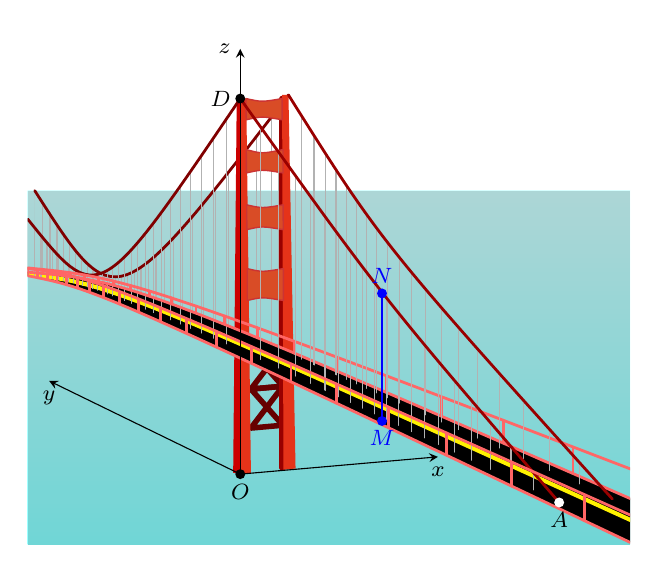
\begin{tikzpicture}[
		scale=0.9, 
		font=\footnotesize, 
		line join=round, 
		line cap=round, 
		>=stealth
		]
		
		\clip (-3,-1) rectangle (5.5,6.3);
		
		\fill[opacity=0.8, bottom color=cyan!50!white, top color=cyan!20!white] 
		(-3,-1) rectangle (5.5,4);
		
		\begin{scope}
			\clip (0.68,5.35) .. controls (-1.75,2.2) .. (-2.9,4) -- 
			(-2.9,2.85) .. controls (-2,2.5) .. (0.68,1.75) -- cycle;
			\foreach \i in {1,2,...,30} {
				\path (0.68,5.35) .. controls (-1.75,2.2) .. (-2.9,4) 
				coordinate[pos=\i/30] (x);
				\draw[gray!60!white] (x) -- ++(-90:4);
			}
		\end{scope}
		
		\draw[red!50!black, line width=1pt] 
		(0.68,5.35) .. controls (-1.75,2.2) .. (-2.9,4);
		
		\draw[line width=2pt, red!40!black] 
		(0.15,0.65) -- (0.6,0.69) -- (0.15,1.2) -- (0.6,1.24) -- cycle;
		\draw[line width=2pt, red!40!black, shift={(0,0.55)}] 
		(0.15,0.65) -- (0.6,0.69) -- (0.15,1.2) -- (0.6,1.24) -- cycle;
		
		\node[brown!40!red, rotate=90] at (0.66,0.5) {1112};
		\draw[red!60!black, line width=2pt] (0.59,0.09) -- (0.59,5.3);
		\fill[brown!40!red] 
		(0.61,0.06) -- (0.59,5.35) -- (0.68,5.35) -- (0.78,0.08) -- cycle;
		
		\fill[brown!40!red] 
		(0,0) coordinate(O) -- (0,5.3) coordinate(D) -- 
		(0.085,5.3) -- (0.15,0.02) -- cycle;
		\fill[black!20!red] 
		(O) -- (D) -- (-0.05,5.32) -- (-0.1,0.02) -- cycle;
		
		\fill[brown!60!red, draw=gray!40!red, line width=0.5pt] 
		(0.08,5.3) .. controls (0.305,5.25) .. (0.59,5.3) -- 
		(0.591,5) .. controls (0.305,5.05) .. (0.084,5) -- cycle;
		\fill[brown!60!red, draw=gray!40!red, line width=0.5pt] 
		(0.085,4.58) .. controls (0.306,4.52) .. (0.603,4.58) -- 
		(0.603,4.25) .. controls (0.3065,4.3) .. (0.086,4.25) -- cycle;
		\fill[brown!60!red, draw=gray!40!red, line width=0.5pt] 
		(0.091,3.8) .. controls (0.307,3.75) .. (0.605,3.8) -- 
		(0.606,3.45) .. controls (0.307,3.5) .. (0.093,3.45) -- cycle;
		\fill[brown!60!red, draw=gray!40!red, line width=0.5pt] 
		(0.098,2.9) .. controls (0.308,2.85) .. (0.608,2.9) -- 
		(0.609,2.45) .. controls (0.308,2.5) .. (0.099,2.45) -- cycle;
		
		\fill (6,-1.2) .. controls (-2,2.6) .. (-3,2.8) -- 
		(-3,2.85) .. controls (-1.5,2.72) .. (7,-1) -- cycle;
		\draw[yellow, line width=1.5pt] 
		(6.5,-1.1) .. controls (-1.75,2.66) .. (-3,2.825);
		
		\def\ipos{20}
		\begin{scope}
			\clip (0,5.3) .. controls (-2,2.35) .. (-3,3.6) -- 
			(-3,2.8) .. controls (-2.2,2.7) .. (0,1.75) -- cycle;
			\foreach \i in {1,2,...,30} {
				\path (0,5.3) .. controls (-2,2.35) .. (-3,3.6) 
				coordinate[pos=\i/30] (y);
				\draw[gray!60!white] (y) -- ++(-90:4);
			}
		\end{scope}
		
		\draw[red!50!black, line width=1pt] 
		(0,5.3) .. controls (-2,2.35) .. (-3,3.6);
		
		\draw[line width=1pt, red!60!white] 
		(7,-1) .. controls (-1.5,2.72) .. (-3,2.85);
		\draw[line width=1pt, red!60!white] 
		(7,-0.5) .. controls (-1.5,2.76) .. (-3,2.91);
		\foreach \t in {1, 2, ..., \ipos} {
			\path (7,-1) coordinate(c) .. controls (-1.5,2.72) .. (-3,2.85) 
			coordinate[pos=\t/\ipos] (d);
			\path (7,-0.5) coordinate(c') .. controls (-1.5,2.76) .. (-3,2.91) 
			coordinate[pos=\t/\ipos] (d');
			\draw[line width=1pt, red!60!white] (d) -- (d');
		}
		
		\begin{scope}
			\clip (D) .. controls (2,2.5) .. (4.5,-0.4) -- (0,1.75) -- cycle;
			\foreach \i in {1,2,...,20} {
				\path (D) .. controls (2,2.5) .. (4.5,-0.4) 
				coordinate[pos=\i/20] (x');
				\draw[gray!60!white] (x') -- ++(-90:4);
			}
		\end{scope}
		
		\begin{scope}
			\clip (0.68,5.35) .. controls (2,3.25) .. (5.25,-0.35) -- 
			(0.68,1.7) -- cycle;
			\foreach \i in {1,2,...,20} {
				\path (0.68,5.35) .. controls (2,3.25) .. (5.25,-0.35) 
				coordinate[pos=\i/20] (y');
				\draw[gray!60!white] (y') -- ++(-90:4);
			}
		\end{scope}
		
		\draw[red!60!black, line width=1pt] 
		(D) .. controls (2,2.5) .. (4.5,-0.4);
		\draw[red!60!black, line width=1pt] 
		(0.68,5.35) .. controls (2,3.25) .. (5.25,-0.35);
		
		\draw[line width=1pt, red!60!white] 
		(6,-1.2) .. controls (-2,2.6) .. (-3,2.8);
		\draw[line width=1pt, red!60!white] 
		(6,-0.8) .. controls (-2,2.78) .. (-3,2.9);
		\foreach \t in {1, 2, ..., \ipos} {
			\path (6,-1.2) coordinate(a) .. controls (-2,2.6) .. (-3,2.8) 
			coordinate[pos=\t/\ipos] (b);
			\path (6,-0.8) coordinate(a') .. controls (-2,2.78) .. (-3,2.9) 
			coordinate[pos=\t/\ipos] (b');
			\draw[line width=1pt, red!60!white] (b) -- (b');
		}
		
		\fill[white] (4.5,-0.4) coordinate(A) node[below, black] {$A$} circle(2pt);
		\fill[blue] (2,0.75) coordinate(M) node[below] {$M$} circle(2pt);
		\fill[blue] (2,2.55) coordinate(N) node[above] {$N$} circle(2pt);
		\draw[blue, line width=1pt] (M) -- (N);
		
		\draw[->] (O) -- (154:3) node[below] {$y$};
		\draw[->] (O) -- (5:2.8) node[below] {$x$};
		\draw[->] (O) -- (90:6) node[left] {$z$};
		
		\fill (O) node[below] {$O$} circle(2pt);
		\fill (D) node[left] {$D$} circle(2pt);
			
	\end{tikzpicture}}
	\choiceTF
	{\True Tọa độ điểm $D$ là $(0;0;227)$}
	{\True Tọa độ của vectơ $\overrightarrow{AD}$ là $(0;-343;152)$}
	{\True Độ dài dây cáp $AD$ là $375{,}17$ m \textit{(kết quả làm tròn đến hàng phần trăm)}}
	{Người ta dùng một đoạn đèn led trang trí nối thẳng từ điểm $N$ trên dây cáp $AD$ đến điểm $M$ trên thành cầu, biết $M$ cách mặt nước $75$ m, cách trục $Oz$ một khoảng bằng $230$ m và $MN$ song song với cột trụ. Độ dài đoạn đèn led cần dùng là $55{,}08$ m \textit{(kết quả làm tròn đến hàng phần trăm)}}
	\loigiai{
		\begin{center}
			\begin{tikzpicture}[scale=0.8, line join=round, line cap=round, >=stealth]
				\def\x{0.6} \def\y{0.8} \def\z{1.5}
				\coordinate (O) at (0,0);
				\coordinate (X) at (-\x,-\y);
				\coordinate (Y) at (6,0);
				\coordinate (Z) at (0,4.5);
				\coordinate (D) at (0,4); % 227m scaled
				\coordinate (A) at (5,1.3); % 343m, 75m scaled
				\coordinate (Az) at (0,1.3);
				\coordinate (Ay) at (5,0);
				
				\draw[->] (O) -- (X) node[below left] {$x$};
				\draw[->] (O) -- (Y) node[below] {$y$};
				\draw[->] (O) -- (Z) node[right] {$z$};
				
				\fill (O) circle (1.5pt) node[below right] {$O$};
				\fill (D) circle (1.5pt) node[left] {$D$};
				\fill (A) circle (1.5pt) node[above] {$A$};
				
				\draw[thick] (D) -- (A);
				\draw[dashed] (A) -- (Az) node[left] {};
				\draw[dashed] (A) -- (Ay) node[below] {};
				
				\draw[gray, thick] (0,1.3) -- (6,1.3);
				
				\coordinate (M) at ($(0,1.3)!0.33!(A)$); % 230m scaled
				\coordinate (N) at ($(D)!0.33!(A)$); % Projection roughly
				\draw[dashed] (M) -- (N);
				\fill (M) circle (1.5pt) node[below] {$M$};
				\fill (N) circle (1.5pt) node[above right] {$N$};
				
				\node[left] at (0,2) {Cột trụ};
				\node[above] at (3.5,2.2) {Dây cáp};
			\end{tikzpicture}
		\end{center}
		\begin{itemchoice}
			\itemch Điểm $D$ thuộc trục $Oz$ và cách mặt nước $227$ m nên $D(0;0;227)$.
			\itemch Điểm $A$ thuộc mặt phẳng $(Oyz)$ nên $x_A=0$, $A$ cách mặt nước $75$ m nên $z_A=75$, $A$ cách trục $Oz$ là $343$ m và nằm ở phía dương trục $Oy$ nên $y_A=343$. Vậy $A(0;343;75)$.\\
			Ta có $\overrightarrow{AD} = (0-0; 0-343; 227-75) = (0; -343; 152)$.
			\itemch Độ dài dây cáp $AD = \sqrt{0^2 + (-343)^2 + 152^2} = \sqrt{117\,649 + 23\,104} = \sqrt{140\,753} \approx 375{,}17$ m.
			\itemch Điểm $M$ trên thành cầu cách mặt nước $75$ m và cách trục $Oz$ là $230$ m nên $M(0; 230; 75)$.\\
			Điểm $N$ thuộc đoạn $AD$ và $MN \parallel Oz$ nên $x_N=x_M=0$ và $y_N=y_M=230$.\\
			Ta có $\overrightarrow{DA} = (0; 343; -152)$. Phương trình tham số đường thẳng $DA$: $\heva{&x=0\\&y=343t\\&z=227-152t}$.\\
			Vì $y_N=230 \Rightarrow 343t=230 \Rightarrow t=\dfrac{230}{343}$.\\
			Suy ra $z_N = 227 - 152 \cdot \dfrac{230}{343} \approx 125{,}08$ m.\\
			Độ dài đoạn đèn led là $MN = |z_N - z_M| = |125{,}08 - 75| = 50{,}08$ m.\\
			Kết quả $55{,}08$ m là sai.
		\end{itemchoice}
	}
\end{ex}

\begin{ex}%[2D1H5-1]
	\immini[thm]
	{Cho hàm số bậc ba $f(x)=ax^3+bx^2+cx+d,\ (a\ne 0)$ liên tục trên $\mathbb{R}$ và có đồ thị như hình vẽ.
	\choiceTF
	{Trong bốn giá trị $a$, $b$, $c$, $d$ có đúng một giá trị bằng $0$}
	{\True Hàm số $y=f(x)$ là hàm số lẻ trên tập $\mathbb{R}$}
	{\True Điểm cực tiểu của đồ thị hàm số $y=f(x)$ là $x=-1$}
	{\True Số nghiệm thực của phương trình $f(x)=\dfrac{2\,025}{2\,026}$ là $3$}}
	{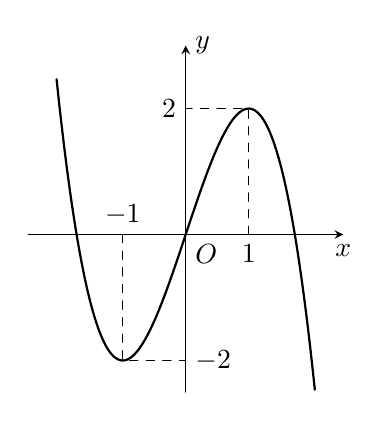
\begin{tikzpicture}[scale=0.8, line join=round, line cap=round, >=stealth]
		\draw[->] (-2.5,0) -- (2.5,0) node[below] {$x$};
		\draw[->] (0,-2.5) -- (0,3) node[right] {$y$};
		\draw (0,0) node[below right] {$O$};
		% Các điểm cực trị (-1, -2) và (1, 2)
		\draw[dashed] (-1,0) node[above]{$-1$} -- (-1,-2) -- (0,-2) node[right]{$-2$};
		\draw[dashed] (1,0) node[below]{$1$} -- (1,2) -- (0,2) node[left]{$2$};
		% Đồ thị hàm số y = -x^3 + 3x
		\draw[thick, smooth, samples=100, domain=-2.05:2.05] plot(\x, {-(\x)^3 + 3*(\x)});
	\end{tikzpicture}}
	\loigiai{
		\begin{itemchoice}
			\itemch Dựa vào đồ thị
			\begin{itemize}
				\item Đồ thị đi qua gốc tọa độ $O(0;0) \Rightarrow d=0$.
				\item Đồ thị nhận gốc tọa độ $O$ làm tâm đối xứng nên là hàm số lẻ $\Rightarrow b=0$.
				\item Hàm số đạt cực trị tại $x=\pm 1$.\\
				Ta có $f'(x) = 3ax^2 + 2bx + c$. Vì $b=0$ nên $f'(x) = 3ax^2 + c$.\\
				$f'(1) = 3a + c = 0 \Rightarrow c = -3a$.\\
				$f(1) = a + c = 2 \Rightarrow a - 3a = 2 \Rightarrow -2a = 2 \Rightarrow a = -1$.\\
				Suy ra $c = 3$.
			\end{itemize}
			Vậy $a=-1$, $b=0$, $c=3$, $d=0$. Có hai giá trị bằng $0$ là $b$ và $d$.
			\itemch Hàm số có $b=0, d=0$ nên $f(x) = -x^3 + 3x$. Ta có $f(-x) = -(-x)^3 + 3(-x) = x^3 - 3x = -f(x)$. Vậy đây là hàm số lẻ.
			\itemch Dựa vào đồ thị, hàm số đạt cực tiểu tại $x=-1$ (tại đó $y=-2$).
			\itemch Phương trình $f(x) = \dfrac{2\,025}{2\,026} \approx 0{,}999$.\\
			Giá trị cực đại là $2$, giá trị cực tiểu là $-2$.\\
			Vì $-2 < 0{,}999 < 2$ nên đường thẳng $y = \dfrac{2\,025}{2\,026}$ cắt đồ thị hàm số tại $3$ điểm phân biệt.
		\end{itemchoice}
	}
\end{ex}

\Closesolutionfile{ans}

\caukq
\Opensolutionfile{ans}[ans/ans\currfilebase-Phan-III]

\begin{ex}%[0D8V2-6]
	Cho một đa giác đều $(H)$ có $15$ đỉnh. Người ta lập một tứ giác có $4$ đỉnh là $4$ đỉnh của $(H)$. Tính số tứ giác được lập thành mà không có cạnh nào là cạnh của $(H)$.
	\par\shortans[oly]{$450$}
	\loigiai{
		Số cách chọn $4$ đỉnh bất kỳ từ $15$ đỉnh của đa giác là $\mathrm{C}_{15}^4$.\\
		Để lập được một tứ giác mà không có cạnh nào là cạnh của đa giác $(H)$, ta thực hiện như sau:\\
		Đánh số các đỉnh của đa giác là $1, 2, \ldots, 15$ theo chiều kim đồng hồ.\\
		Giả sử $4$ đỉnh được chọn là $x_1$, $x_2$, $x_3$, $x_4$ với $1 \le x_1 < x_2 < x_3 < x_4 \le 15$.\\
		Điều kiện để không có cạnh nào của tứ giác là cạnh của đa giác là\\
		$x_{i+1} - x_i \ge 2$ với $i=1,2,3$ và $15 - x_4 + x_1 \ge 2$ (để tránh cặp đỉnh $15$ và $1$).\\
		Theo bài toán chia kẹo Euler hoặc công thức chọn $k$ phần tử từ $n$ phần tử xếp vòng tròn sao cho không có $2$ phần tử nào kề nhau, số cách chọn là $\dfrac{n}{n-k} \mathrm{C}_{n-k}^k$ với $n=15$, $k=4$.\\
		Số tứ giác thỏa mãn là $\dfrac{15}{15-4}\cdot  \mathrm{C}_{15-4}^4 = \dfrac{15}{11}\cdot  \mathrm{C}_{11}^4 = \dfrac{15}{11} \cdot 330 = 450$.\\
		Vậy có $450$ tứ giác thỏa mãn yêu cầu bài toán.
	}
\end{ex}

\begin{ex}%[1H8V7-6]
	\immini[thm]
	{Một chậu đựng nước có dạng hình chóp cụt tứ giác đều với chiều cao $3$ dm, cạnh đáy lần lượt là $2$ dm và $4$ dm. Người ta bơm nước vào chậu với lưu lượng không đổi $4{,}75$ lít/phút. Hỏi sau $2$ phút chiều cao nước trong chậu là bao nhiêu dm, biết lúc đầu chậu không chứa nước?}
	{\begin{tikzpicture}[line join=round, line cap=round, >=stealth, scale=0.5]
		\coordinate (A) at (-1.5, 0);
		\coordinate (B) at (1.5, 0);
		\coordinate (C) at (2.3, 1);
		\coordinate (D) at (-0.7, 1);
		\coordinate (A') at (-2.5, 4);
		\coordinate (B') at (2.5, 4);
		\coordinate (C') at (3.8, 5);
		\coordinate (D') at (-1.2, 5);
		\coordinate (M) at ($(A)!0.6!(A')$);
		\coordinate (N) at ($(B)!0.6!(B')$);
		\coordinate (P) at ($(C)!0.6!(C')$);
		\coordinate (Q) at ($(D)!0.6!(D')$);
		\fill[cyan!30, opacity=0.6] (A)--(B)--(N)--(M)--cycle; % Mặt trước
		\fill[cyan!50, opacity=0.6] (B)--(C)--(P)--(N)--cycle; % Mặt bên phải
		\fill[cyan!20, opacity=0.6] (M)--(N)--(P)--(Q)--cycle; % Mặt thoáng
		\draw[dashed] (A)--(D)--(C); % AD và DC
		\draw[dashed] (D)--(D');     % DD'
		\draw[blue!80, dashed] (M)--(Q)--(P);
		\draw (A)--(B)--(C);
		\draw (A)--(A') (B)--(B') (C)--(C');
		\draw (A')--(B')--(C')--(D')--cycle;
		\draw[blue!80, thick] (M)--(N)--(P);
	\end{tikzpicture}}
	\par\shortans[oly]{$1{,}5$}
	\loigiai{
		\immini
		{Đổi đơn vị $1$ lít $= 1$ dm$^3$.\\
		Lượng nước bơm vào sau $2$ phút là $V_{\text{nước}} = 4{,}75 \times 2 = 9{,}5$ dm$^3$.\\
		Vì chậu nước có dạng hình chóp cụt tứ giác đều, nên phần nước chứa trong chậu cũng là một khối chóp cụt tứ giác đều.\\
		Gọi $h$ là chiều cao của mực nước ($h>0$).\\
		Cạnh đáy dưới của chậu (nhỏ hơn) là $a=2$ dm. Cạnh đáy trên của chậu (lớn hơn) là $b=4$ dm. Chiều cao chậu là $H=3$ dm.\\
		Cạnh của mặt nước hình vuông tại độ cao $h$ là $x$ dm.}
		{\begin{tikzpicture}[line join=round, line cap=round, >=stealth, scale=0.7]
				\coordinate (A) at (0,0);
				\coordinate (B) at (6,0);
				\coordinate (D) at (1.2, 1.5); 
				\coordinate (C) at ($(B)+(D)-(A)$); % C = B + D - A
				\coordinate (O) at ($(A)!0.5!(C)$);
				\coordinate (Op) at ($(O)+(0, 4.5)$); % Tâm đáy trên O'
				\def\k{0.5}
				\coordinate (Ap) at ($(Op)+\k*(A)-\k*(O)$); % A'
				\coordinate (Bp) at ($(Op)+\k*(B)-\k*(O)$); % B'
				\coordinate (Cp) at ($(Op)+\k*(C)-\k*(O)$); % C'
				\coordinate (Dp) at ($(Op)+\k*(D)-\k*(O)$); % D'
				\def\t{0.4}
				\coordinate (A1) at ($(A)!\t!(Ap)$);
				\coordinate (B1) at ($(B)!\t!(Bp)$);
				\coordinate (C1) at ($(C)!\t!(Cp)$);
				\coordinate (D1) at ($(D)!\t!(Dp)$);
				\coordinate (H) at ($(O)+\k*(A)-\k*(O)$);
				\coordinate (K) at (intersection of Ap--H and A1--C1);
				\draw[blue, dashed] (A)--(D) (D)--(C) (D)--(Dp); % Cạnh đáy và bên khuất
				\draw[blue, dashed] (A1)--(D1) (D1)--(C1); % Cạnh mặt cắt khuất
				\draw[blue, dashed] (A)--(C) (B)--(D); % Đường chéo đáy dưới
				\draw[blue, dashed] (A1)--(C1) (B1)--(D1); % Đường chéo mặt cắt
				\draw[blue, dashed] (Ap)--(H); % Đường vuông góc A'H
				\draw[blue, thick] (A)--(B)--(C); % Đáy dưới
				\draw[blue, thick] (A)--(Ap) (B)--(Bp) (C)--(Cp); % Cạnh bên
				\draw[blue, thick] (Ap)--(Bp)--(Cp)--(Dp)--cycle; % Đáy trên
				\draw[blue, thick] (Ap)--(Cp) (Bp)--(Dp); % Đường chéo đáy trên (thấy)
				\draw[blue, thick] (A1)--(B1)--(C1); % Mặt cắt (phần thấy)
				\foreach \p in {A,B,C,D,Ap,Bp,Cp,Dp,A1,B1,C1,D1,H,K}
				\fill[red] (\p) circle (1.5pt);
				\node[left] at (A) {$A$};
				\node[right] at (B) {$B$};
				\node[right] at (C) {$C$};
				\node[left] at (D) {$D$};
				
				\node[left] at (Ap) {$A'$};
				\node[right] at (Bp) {$B'$};
				\node[right] at (Cp) {$C'$};
				\node[left] at (Dp) {$D'$};
				
				\node[left] at (A1) {$A_1$};
				\node[right] at (B1) {$B_1$};
				\node[right] at (C1) {$C_1$};
				\node[left] at (D1) {$D_1$};
				
				\node[below] at (H) {$H$};
				\node[above right] at (K) {$K$};
				
		\end{tikzpicture}}
		\noindent
		Ta có tỉ lệ $\dfrac{x-a}{b-a} = \dfrac{h}{H} \Rightarrow \dfrac{x-2}{4-2} = \dfrac{h}{3} \Rightarrow \dfrac{x-2}{2} = \dfrac{h}{3} \Rightarrow h = \dfrac{3(x-2)}{2}$.\\
		Thể tích nước là thể tích khối chóp cụt có hai đáy là $a$ và $x$, chiều cao $h$ là\\
		\[V = \dfrac{1}{3}h(a^2 + x^2 + ax) = \dfrac{1}{3} \cdot \dfrac{3(x-2)}{2} \cdot (2^2 + x^2 + 2x) = \dfrac{x-2}{2}(x^2+2x+4) = \dfrac{x^3 - 8}{2}.\]
		Theo bài ra ta có $\dfrac{x^3 - 8}{2} = 9{,}5 \Leftrightarrow x^3 - 8 = 19 \Leftrightarrow x^3 = 27 \Leftrightarrow x = 3$ (dm).\\
		Khi đó chiều cao nước là $h = \dfrac{3(3-2)}{2} = 1{,}5$ (dm).\\
		Vậy chiều cao nước trong chậu là $1{,}5$ dm.
	}
\end{ex}

\begin{ex}%[0D0V2-5]
	Hai bạn Hải và Sơn cùng chơi một trò chơi như sau: Hải có một hộp gồm $9$ quả bóng được đánh số từ $1$ đến $9$, Sơn có một hộp gồm $8$ quả bóng được đánh số từ $1$ đến $8$. Mỗi bạn bốc ngẫu nhiên $3$ quả bóng từ hộp của mình rồi xếp các số ghi trên $3$ quả bóng bốc được theo thứ tự giảm dần để tạo thành một số có $3$ chữ số. Bạn nào có số lớn hơn là người chiến thắng. Tính xác suất để Sơn thua (kết quả làm tròn đến hàng phần trăm).
	\par\shortans[oly]{$0{,}66$}
	\loigiai{
		Số phần tử của không gian mẫu là $n(\Omega) = \mathrm{C}_9^3 \cdot \mathrm{C}_8^3 = 84 \cdot 56 = 4\,704$.\\
		Gọi $A$ là biến cố \lq\lq Sơn thua\rq\rq\, tức là số của Sơn nhỏ hơn số của Hải.\\
		Gọi bộ $3$ quả bóng Hải bốc được là $H=\{h_1, h_2, h_3\}$ với $h_1 > h_2 > h_3$.\\
		Gọi bộ $3$ quả bóng Sơn bốc được là $S=\{s_1, s_2, s_3\}$ với $s_1 > s_2 > s_3$.\\
		Số của Hải là $\overline{h_1h_2h_3}$, số của Sơn là $\overline{s_1s_2s_3}$.\\
		Xét hai trường hợp\\
		\textbf{Trường hợp 1}. Hải bốc được quả bóng số $9$ ($h_1=9$).\\
		Khi đó số của Hải chắc chắn lớn hơn số của Sơn (vì số của Sơn có chữ số hàng trăm tối đa là $8$).\\
		Số cách chọn của Hải là $1 \cdot \mathrm{C}_8^2 = 28$ cách.\\
		Số cách chọn của Sơn là $\mathrm{C}_8^3 = 56$ cách.\\
		Số kết quả thuận lợi là $28 \cdot 56 = 1568$.\\
		\textbf{Trường hợp 2}. Hải không bốc được quả bóng số $9$.\\
		Lúc này Hải bốc $3$ quả từ tập $\{1; 2; \ldots; 8\}$, Sơn cũng bốc $3$ quả từ tập $\{1; 2; \ldots; 8\}$.\\
		Tổng số cách chọn trong trường hợp này là $\mathrm{C}_8^3 \cdot \mathrm{C}_8^3 = 56 \cdot 56 = 3\,136$.\\
		Trong trường hợp này, vai trò của Hải và Sơn là như nhau. Có $3$ khả năng: Hải thắng, Sơn thắng, Hòa.\\
		Số trường hợp Hòa (hai bạn bốc y hệt nhau) là $\mathrm{C}_8^3 = 56$.\\
		Số trường hợp Hải thắng bằng số trường hợp Sơn thắng: $\dfrac{3\,136 - 56}{2} = 1\,540$.\\
		Số kết quả thuận lợi cho biến cố $A$ là $n(A) = 1\,568 + 1\,540 = 3\,108$.\\
		Xác suất cần tìm là $\mathrm{P}(A) = \dfrac{3\,108}{4\,704} \approx 0{,}66$.
	}
\end{ex}

\begin{ex}%[2D1V3-5]
	Cho hàm số $y=x^3-3(m+1)x^2+3(m^2+2m)x-2\,025$ với $m$ là tham số. Có bao nhiêu giá trị nguyên của tham số $m$ để hàm số có giá trị lớn nhất trên khoảng $(-\infty;0)$?
	\par\shortans[oly]{$3$}
	\loigiai{
		Ta có $y'=3x^2-6(m+1)x+3(m^2+2m)$.\\
		$y'=0 \Leftrightarrow x^2-2(m+1)x+m(m+2)=0 \Leftrightarrow \hoac{&x=m\\ &x=m+2.}$\\
		Vì $m < m+2$ nên hàm số đạt cực đại tại $x=m$ và cực tiểu tại $x=m+2$.\\
		Bảng biến thiên:
		\begin{center}
			
\begin{tikzpicture}
				\tkzTabInit[lgt=1.2,espcl=2.5]
				{$x$ /1, $y'$ /1, $y$ /2}
				{$-\infty$, $m$, $m+2$, $+\infty$}
				\tkzTabLine{,+,0,-,0,+,}
				\tkzTabVar{-/ $-\infty$, +/ $y(m)$, -/ $y(m+2)$, +/ $+\infty$}
			\end{tikzpicture}
		\end{center}
		Dựa vào bảng biến thiên, trên khoảng $(-\infty; 0)$ hàm số có giá trị lớn nhất khi và chỉ khi:\\
		$\heva{&m < 0\\ &y(m) \ge y(0)}$ (trong trường hợp $m+2 < 0$, đồ thị đi xuống rồi đi lên đến $0$, cần đỉnh cực đại cao hơn hoặc bằng giá trị tại biên $0$).\\
		Hoặc trường hợp đơn giản là $m < 0 \le m+2$, khi đó trên $(-\infty; 0)$ hàm số đồng biến đến $m$ rồi nghịch biến, nên giá trị lớn nhất chính là $y(m)$.\\
		Xét cụ thể\\
		$y(m) = m^3 - 3(m+1)m^2 + 3(m^2+2m)m - 2\,025 = m^3 + 3m^2 - 2\,025$.\\
		$y(0) = -2\,025$.\\
		Điều kiện $y(m) \ge y(0) \Leftrightarrow m^3 + 3m^2 - 2\,025 \ge -2\,025 \Leftrightarrow m^2(m+3) \ge 0 \Leftrightarrow m \ge -3$.\\
		Kết hợp các trường hợp
		\begin{itemize}
			\item Nếu $m < 0 \le m+2 \Leftrightarrow -2 \le m < 0$: hàm số đạt giá trị lớn nhất tại $x=m$ (thỏa mãn).
			\item Nếu $m+2 < 0 \Leftrightarrow m < -2$: hàm số đạt giá trị lớn nhất trên $(-\infty; 0)$ khi $y(m) \ge \lim\limits_{x \to 0^-} y(x) = y(0)$.\\
				Khi đó cần $m \ge -3$, vậy $-3 \le m < -2$.
		\end{itemize}
		Tóm lại, giá trị $m$ thỏa mãn là $-3 \le m < 0$.\\
		Vì $m \in \mathbb{Z}$ nên $m \in \{-3; -2; -1\}$.\\
		Vậy có $3$ giá trị nguyên của tham số $m$ thỏa mãn.
	}
\end{ex}

\begin{ex}%[2H2V2-6]
	Một căn phòng có dạng hình hộp chữ nhật với chiều dài $4$ m, chiều rộng $3$ m và chiều cao $3$ m. Xét hệ trục tọa độ $Oxyz$ có gốc $O$ trùng với một góc phòng và mặt phẳng $(Oxy)$ trùng với mặt sàn (xem hình vẽ), đơn vị đo được lấy theo mét. Trên bức tường thuộc mặt phẳng $(Oyz)$ có một cột dạng hình hộp chữ nhật nhô ra với chiều dài $0{,}4$ m, chiều rộng $0{,}2$ m. Bác Nam lắp một bóng đèn trên tường tại vị trí điểm $A(1;0;2{,}5)$ và công tắc bóng đèn đặt tại điểm $B(0{,}5;4;1)$. Dây cấp điện cho bóng đèn được đấu từ công tắc điện dọc theo các bức tường (không đi qua trần nhà, sàn nhà) và nối đến bóng đèn. Hỏi bác phải dùng đoạn dây điện có độ dài tối thiểu là bao nhiêu mét \textit{(kết quả làm tròn đến hàng phần trăm)}?
	\begin{center}
		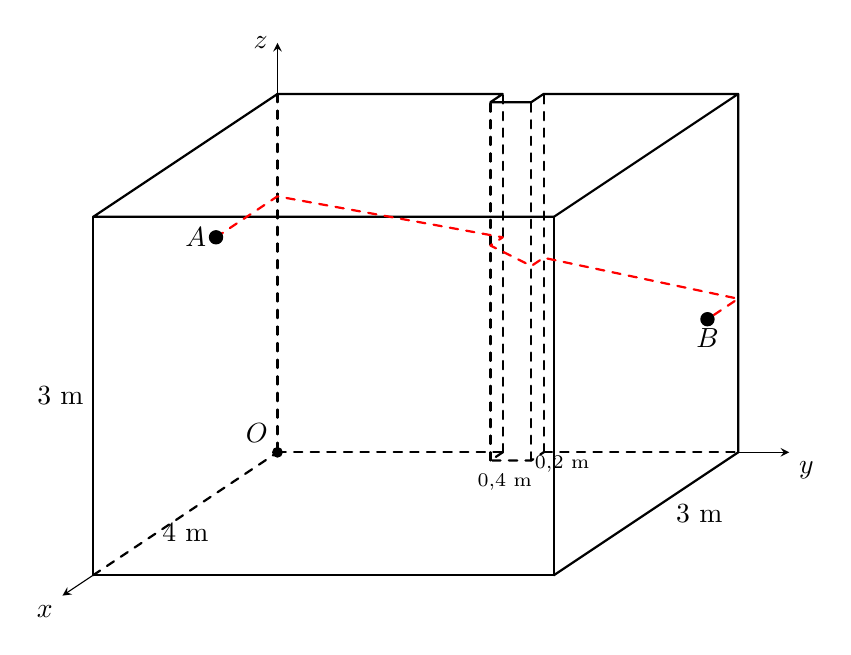
\begin{tikzpicture}[line join=round, line cap=round, >=stealth, scale=1.3, x={(-0.6cm,-0.4cm)}, y={(1cm,0cm)}, z={(0cm,1cm)}]
			\coordinate (O) at (0,0,0);
			\def\L{4.5}
			\def\W{3}
			\def\H{3.5}
			\coordinate (LTB) at (0,0,\H);
			\coordinate (LBB) at (0,0,0);
			\coordinate (RBB) at (0,\L,0);
			\coordinate (RTB) at (0,\L,\H);
			
			\coordinate (LTF) at (\W,0,\H);
			\coordinate (LBF) at (\W,0,0);
			\coordinate (RBF) at (\W,\L,0);
			\coordinate (RTF) at (\W,\L,\H);
			
			\def\pys{2.2}
			\def\pye{2.6}
			\def\px{0.4}
			\def\pw{0.4}
			\def\pd{0.2}
			\coordinate (P1) at (0,\pys,0);
			\coordinate (P2) at (\pd,\pys,0);
			\coordinate (P3) at (\pd,\pye,0);
			\coordinate (P4) at (0,\pye,0);
			\coordinate (P1t) at (0,\pys,\H);
			\coordinate (P2t) at (\pd,\pys,\H);
			\coordinate (P3t) at (\pd,\pye,\H);
			\coordinate (P4t) at (0,\pye,\H);
			\coordinate (A) at (1,0,2.5);
			\coordinate (B) at (0.5,\L,1.5);
			\draw[->] (LBF) -- (\W+0.5,0,0) node[below left] {$x$};
			\draw[->] (RBB) -- (0,\L+0.5,0) node[below right] {$y$};
			\draw[->] (LTB) -- (0,0,\H+0.5) node[left] {$z$};
			\draw[dashed, thick] (LTB) -- (O);
			\draw[dashed, thick] (LBF) -- (O); 
			\draw[dashed, thick] (O) -- (P1);
			\draw[dashed, thick] (P1) -- (P2) -- (P3) -- (P4);
			\draw[dashed, thick] (P4) -- (RBB);
			\draw[dashed, thick] (P1) -- (P1t);
			\draw[dashed, thick] (P2) -- (P2t);
			\draw[dashed, thick] (P3) -- (P3t);
			\draw[dashed, thick] (P4) -- (P4t);
			\draw[thick] (LTB) -- (P1t) -- (P2t) -- (P3t) -- (P4t) -- (RTB) -- (RTF) -- (LTF) -- cycle;
			\draw[thick] (LBF) -- (LTF);
			\draw[thick] (RBF) -- (RTF);
			\draw[thick] (LBF) -- (RBF);
			\draw[thick] (RBF)--(RBB)--(RTB);
			\coordinate (D1) at (0, 0, 2.5);
			\coordinate (D2) at (0, \pys, 2.1);
			\coordinate (D3) at (\pd, \pys, 2.1);
			\coordinate (D4) at (\pd, \pye, 1.9);
			\coordinate (D5) at (0, \pye, 1.9);
			\coordinate (D6) at (0, \L, 1.5);
			
			\draw[thick, dashed, red] (A) -- (D1) -- (D2) -- (D3) -- (D4) -- (D5) -- (D6) -- (B);
			
			\fill (O) circle (1.5pt) node[above left] {$O$};
			\fill (A) circle (2pt) node[left] {$A$};
			\fill (B) circle (2pt) node[below] {$B$};
			
			\node at (3, 0, \H/2) [left] {$3$ m};
			\node at (\W/2, \L+0.2, 0) [right] {$3$ m};
			\node at (\W/2, 0, 0) [below] {$4$ m};
			
			\node at (\pd + 0.1, \pys/2 + \pye/2, 0) [below, font=\scriptsize] {$0{,}4$ m};
			\node at (\pd + 0.1, \pye, 0) [right, font=\scriptsize] {$0{,}2$ m};
			
		\end{tikzpicture}
	\end{center}
	\par\shortans[oly]{$6{,}09$}
	\loigiai{
		Gọi các đỉnh của dây điện như hình vẽ
		\begin{center}
			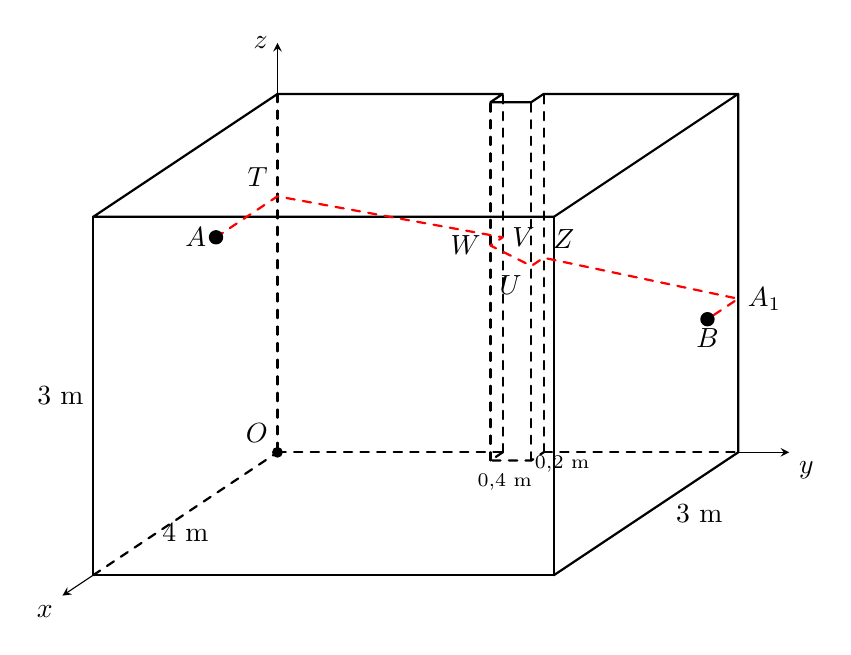
\begin{tikzpicture}[line join=round, line cap=round, >=stealth, scale=1.3, x={(-0.6cm,-0.4cm)}, y={(1cm,0cm)}, z={(0cm,1cm)}]
				\coordinate (O) at (0,0,0);
				
				\def\L{4.5}
				\def\W{3}
				\def\H{3.5}
				
				\coordinate (LTB) at (0,0,\H);
				\coordinate (LBB) at (0,0,0);
				\coordinate (RBB) at (0,\L,0);
				\coordinate (RTB) at (0,\L,\H);
				
				\coordinate (LTF) at (\W,0,\H);
				\coordinate (LBF) at (\W,0,0);
				\coordinate (RBF) at (\W,\L,0);
				\coordinate (RTF) at (\W,\L,\H);
				
				\def\pys{2.2}
				\def\pye{2.6}
				\def\px{0.4}
				\def\pw{0.4}
				\def\pd{0.2}
				
				\coordinate (P1) at (0,\pys,0);
				\coordinate (P2) at (\pd,\pys,0);
				\coordinate (P3) at (\pd,\pye,0);
				\coordinate (P4) at (0,\pye,0);
				
				\coordinate (P1t) at (0,\pys,\H);
				\coordinate (P2t) at (\pd,\pys,\H);
				\coordinate (P3t) at (\pd,\pye,\H);
				\coordinate (P4t) at (0,\pye,\H);
				
				\coordinate (A) at (1,0,2.5);
				\coordinate (B) at (0.5,\L,1.5);
				
				\draw[->] (LBF) -- (\W+0.5,0,0) node[below left] {$x$};
				\draw[->] (RBB) -- (0,\L+0.5,0) node[below right] {$y$};
				\draw[->] (LTB) -- (0,0,\H+0.5) node[left] {$z$};
				
				\draw[dashed, thick] (LTB) -- (O);
				\draw[dashed, thick] (LBF) -- (O); 
				
				\draw[dashed, thick] (O) -- (P1);
				\draw[dashed, thick] (P1) -- (P2) -- (P3) -- (P4); % Chân cột
				\draw[dashed, thick] (P4) -- (RBB);
				
				\draw[dashed, thick] (P1) -- (P1t);
				\draw[dashed, thick] (P2) -- (P2t);
				\draw[dashed, thick] (P3) -- (P3t);
				\draw[dashed, thick] (P4) -- (P4t);
				
				\draw[thick] (LTB) -- (P1t) -- (P2t) -- (P3t) -- (P4t) -- (RTB) -- (RTF) -- (LTF) -- cycle;
				
				\draw[thick] (LBF) -- (LTF);
				\draw[thick] (RBF) -- (RTF);
				\draw[thick] (LBF) -- (RBF);
				\draw[thick] (RBF)--(RBB)--(RTB);
				
				\coordinate[label=above left:$T$] (D1) at (0, 0, 2.5);
				\coordinate[label=right:$V$] (D2) at (0, \pys, 2.1);
				\coordinate[label=left:$W$] (D3) at (\pd, \pys, 2.1);
				\coordinate[label=below left:$U$] (D4) at (\pd, \pye, 1.9);
				\coordinate[label=above right:$Z$] (D5) at (0, \pye, 1.9);
				\coordinate[label=right:$A_1$] (D6) at (0, \L, 1.5);
				
				\draw[thick, dashed, red] (A) -- (D1) -- (D2) -- (D3) -- (D4) -- (D5) -- (D6) -- (B);
				
				\fill (O) circle (1.5pt) node[above left] {$O$};
				\fill (A) circle (2pt) node[left] {$A$};
				\fill (B) circle (2pt) node[below] {$B$};
				
				\node at (3, 0, \H/2) [left] {$3$ m};
				\node at (\W/2, \L+0.2, 0) [right] {$3$ m};
				\node at (\W/2, 0, 0) [below] {$4$ m};
				
				\node at (\pd + 0.1, \pys/2 + \pye/2, 0) [below, font=\scriptsize] {$0{,}4$ m};
				\node at (\pd + 0.1, \pye, 0) [right, font=\scriptsize] {$0{,}2$ m};
				
			\end{tikzpicture}
		\end{center}
		Để tìm độ dài ngắn nhất của dây điện đi dọc theo các bức tường, ta thực hiện "trải phẳng" các bề mặt tường liên quan thành một mặt phẳng.\\
		Theo đề bài và hình vẽ, điểm $A(1;0;2{,}5)$ nằm trên mặt phẳng $Oxz$ (tường bên trái), cách trục $Oz$ một khoảng $x_A=1$ m và cách sàn $z_A=2{,}5$ m.\\
		Điểm $B(0{,}5;4;1)$ nằm ở khu vực tường đối diện hoặc tường bên, nhưng do có tọa độ $y=4$ và sự xuất hiện của cột nhô ra, ta mô hình hóa đường đi trên mặt phẳng trải rộng như hình vẽ
		\begin{center}
			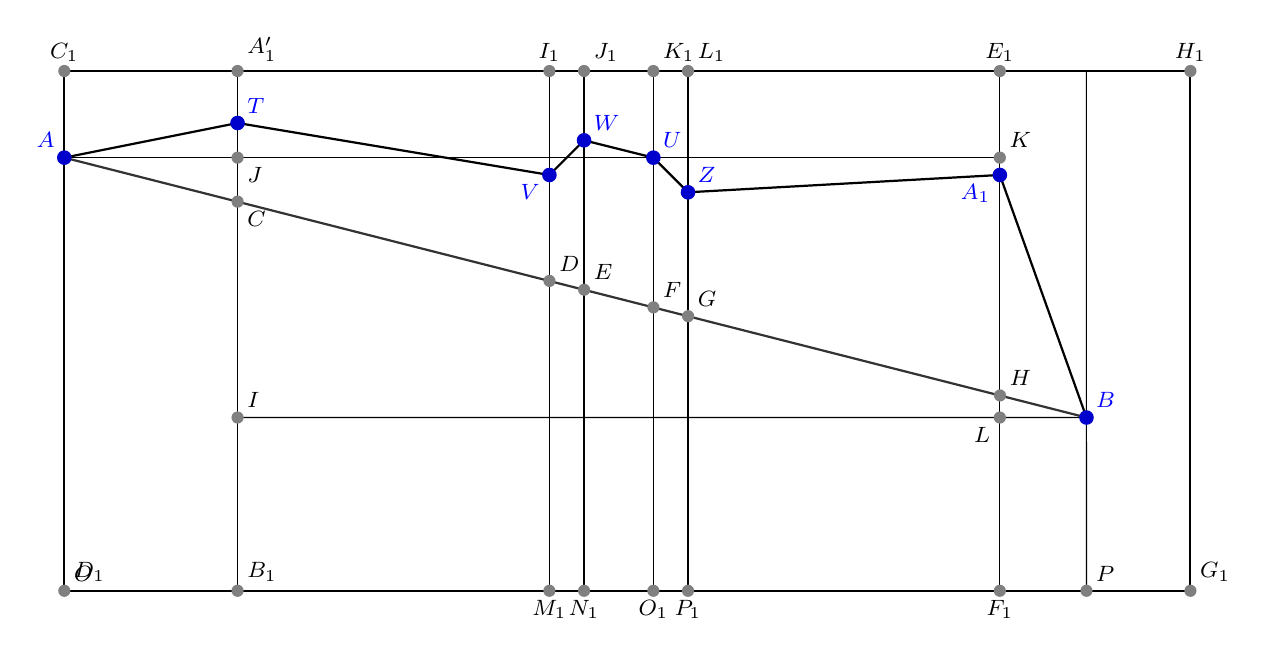
\begin{tikzpicture}[scale=2.2, font=\footnotesize, line join=round, line cap=round, >=stealth]
				\def\h{3}
				\def\zA{2.5}
				\def\zB{1}
				\coordinate (O) at (0,0);
				\coordinate (B1) at (1,0);
				\coordinate (M1) at (2.8,0);
				\coordinate (N1) at (3.0,0);
				\coordinate (O1) at (3.4,0);
				\coordinate (P1) at (3.6,0);
				\coordinate (F1) at (5.4,0);
				\coordinate (P) at (5.9,0);
				\coordinate (G1) at (6.5,0);
				\coordinate (C1) at (0,\h);
				\coordinate (A1p) at (1,\h);
				\coordinate (I1) at (2.8,\h);
				\coordinate (J1) at (3.0,\h);
				\coordinate (K1) at (3.4,\h);
				\coordinate (L1) at (3.6,\h);
				\coordinate (E1) at (5.4,\h);
				\coordinate (H1) at (6.5,\h);
				\coordinate (A) at (0,\zA);
				\coordinate (B) at (5.9,\zB);
				\draw[thick] (0,0) -- (6.5,0);
				\draw[thick] (0,\h) -- (6.5,\h);
				\draw[thick] (0,0) -- (0,\h);
				\draw[thick] (6.5,0) -- (6.5,\h);
				\draw (B1) -- (A1p);
				\draw (M1) -- (I1);
				\draw (N1) -- (J1);
				\draw (O1) -- (K1);
				\draw (P1) -- (L1);
				\draw (F1) -- (E1);
				\draw (P) -- (5.9,\h);
				\draw[thick, black!80] (A) -- (B);
				\coordinate (C) at (intersection of A--B and B1--A1p);
				\coordinate (D) at (intersection of A--B and M1--I1);
				\coordinate (E) at (intersection of A--B and N1--J1);
				\coordinate (F) at (intersection of A--B and O1--K1);
				\coordinate (G) at (intersection of A--B and P1--L1);
				\coordinate (H) at (intersection of A--B and F1--E1);
				\coordinate (T) at (1, 2.7);
				\coordinate (V) at (2.8, 2.4);
				\coordinate (W) at (3.0, 2.6);
				\coordinate (U) at (3.4, 2.5);
				\coordinate (Z) at (3.6, 2.3);
				\coordinate (A1) at (5.4, 2.4);				
				\draw[thick] (A) -- (T) -- (V) -- (W) -- (U) -- (Z) -- (A1) -- (B);
				\coordinate (J) at (1, \zA);
				\coordinate (K) at (5.4, \zA);
				\draw[thin] (A) -- (K);
				\coordinate (I) at (1, 1);
				\coordinate (L) at (5.4, 1);
				\coordinate (B_left) at (0, 1);
				\draw[thin] (1,1) -- (B); 
				\draw[thin] (1,1) -- (1, \zA);
				\draw[thin] (5.4,1) -- (5.4, \zA);
				\foreach \p in {A, T, V, W, U, Z, A1, B}
				\fill[blue!80!black] (\p) circle (1.2pt);
				\foreach \p in {C, D, E, F, G, H, J, K, I, L, O, B1, M1, N1, O1, P1, F1, P, G1, C1, A1p, I1, J1, K1, L1, E1, H1}
				\fill[gray] (\p) circle (1pt);
				\node[above left, blue] at (A) {$A$};
				\node[above right, blue] at (B) {$B$};
				\node[above right, blue] at (T) {$T$};
				\node[below left, blue] at (V) {$V$};
				\node[above right, blue] at (W) {$W$};
				\node[above right, blue] at (U) {$U$};
				\node[above right, blue] at (Z) {$Z$};
				\node[below left, blue] at (A1) {$A_1$};
				\node[below right] at (C) {$C$};
				\node[above right] at (D) {$D$};
				\node[above right] at (E) {$E$};
				\node[above right] at (F) {$F$};
				\node[above right] at (G) {$G$};
				\node[above right] at (H) {$H$};				
				\node[below right] at (J) {$J$};
				\node[above right] at (K) {$K$};
				\node[above right] at (I) {$I$};
				\node[below left] at (L) {$L$};
				\node[above] at (C1) {$C_1$};
				\node[above right] at (A1p) {$A_1'$};
				\node[above] at (I1) {$I_1$};
				\node[above right] at (J1) {$J_1$};
				\node[above right] at (K1) {$K_1$};
				\node[above right] at (L1) {$L_1$};
				\node[above] at (E1) {$E_1$};
				\node[above] at (H1) {$H_1$};
				\node[above right] at (0,0) {$D_1$};
				\node[above right] at (O) {$O$};
				\node[above right] at (B1) {$B_1$};
				\node[below] at (M1) {$M_1$};
				\node[below] at (N1) {$N_1$};
				\node[below] at (O1) {$O_1$};
				\node[below] at (P1) {$P_1$};
				\node[below] at (F1) {$F_1$};
				\node[above right] at (P) {$P$};
				\node[above right] at (G1) {$G_1$};				
			\end{tikzpicture}
		\end{center}
		Gọi $O'$ là hình chiếu của $A$ lên phương thẳng đứng tại mép tường, $P$ là hình chiếu của $B$ lên phương thẳng đứng tương ứng trên mặt phẳng trải.\\
		Khi trải phẳng, khoảng cách ngang giữa $A$ và $B$ bao gồm:
		\begin{itemize}
			\item Khoảng cách từ $A$ đến góc tường $O$: $1$ m.
			\item Chiều dài bức tường $Oyz$ cộng thêm phần chu vi của cột nhô ra. Chiều dài tường là $4$ m. Cột nhô ra có kích thước $0{,}4 \times 0{,}2$. Khi trải phẳng, phần dây đi qua cột sẽ đi theo bề mặt cột, do đó chiều dài ngang tăng thêm $2 \times 0{,}2 = 0{,}4$ m (hai cạnh bên của cột). Tổng chiều dài đoạn giữa là $4 + 0{,}4 = 4{,}4$ m.
			\item Khoảng cách từ $B$ đến mép tường tương ứng (theo tọa độ $x$ hoặc $y$ trong hệ quy chiếu cục bộ của $B$): $0{,}5$ m.
		\end{itemize}
		Tổng khoảng cách theo phương ngang (trên mặt phẳng trải) là
		$L_x = 1 + 4{,}4 + 0{,}5 = 5{,}9$ m.\\
		Khoảng cách theo phương đứng (chênh lệch độ cao):
		$L_z = |z_A - z_B| = |2{,}5 - 1| = 1{,}5$ m.\\
		Độ dài đoạn dây điện tối thiểu là độ dài đoạn thẳng $AB$ trên mặt phẳng trải
		\[L = \sqrt{L_x^2 + L_z^2} = \sqrt{5{,}9^2 + 1{,}5^2} = \sqrt{34{,}81 + 2{,}25} = \sqrt{37{,}06} \approx 6{,}0877.\]
		Làm tròn đến hàng phần trăm, ta được $6{,}09$ m.
	}
\end{ex}

\begin{ex}%[1D6C2-5]
	Với $a$, $b$, $c$ là các số thực thỏa mãn $\dfrac{1}{3} < a < 1$; $\dfrac{1}{3} < b < 1$; $\dfrac{1}{8} < c < 1$. Tính giá trị nhỏ nhất của biểu thức $P=4\log_{a}\left(\dfrac{3b-1}{4}\right)+3\log_{b}\left(\dfrac{c}{2}-\dfrac{1}{16}\right)+6\log_{c}\left(\dfrac{a}{2}-\dfrac{3}{16}\right)$.
	\par\shortans[oly]{$36$}
	\loigiai{
		Ta có nhận xét sau $b^3 - \dfrac{3b-1}{4} = \dfrac{4b^3 - 3b + 1}{4} = \dfrac{(b+1)(2b-1)^2}{4}$.\\
		Vì $\dfrac{1}{3} < b < 1$ nên $b+1 > 0$, suy ra $b^3 \ge \dfrac{3b-1}{4}$ (dấu \lq\lq$=$\rq\rq\, xảy ra khi $b=\dfrac{1}{2}$).\\
		Vì $\dfrac{1}{3} < a < 1$ nên hàm số $y = \log_a x$ nghịch biến. Do đó
		$4\log_a\left(\dfrac{3b-1}{4}\right) \ge 4\log_a(b^3) = 12\log_a b$. \quad (1)\\
		Tương tự, xét $c^2 - \left(\dfrac{c}{2}-\dfrac{1}{16}\right) = c^2 - \dfrac{c}{2} + \dfrac{1}{16} = \left(c-\dfrac{1}{4}\right)^2 \ge 0 \Rightarrow c^2 \ge \dfrac{c}{2}-\dfrac{1}{16}$.\\
		Vì $\dfrac{1}{3} < b < 1$ nên $3\log_b\left(\dfrac{c}{2}-\dfrac{1}{16}\right) \ge 3\log_b(c^2) = 6\log_b c$. \quad (2)\\
		Xét $a^4 - \left(\dfrac{a}{2}-\dfrac{3}{16}\right) = a^4 - \dfrac{a}{2} + \dfrac{3}{16}$.\\
		Phân tích $a^4 - \dfrac{a}{2} + \dfrac{3}{16} = \left(a-\dfrac{1}{2}\right)^2 \left(a^2+a+\dfrac{3}{4}\right) \ge 0 \Rightarrow a^4 \ge \dfrac{a}{2}-\dfrac{3}{16}$.\\
		Vì $\dfrac{1}{8} < c < 1$ nên $6\log_c\left(\dfrac{a}{2}-\dfrac{3}{16}\right) \ge 6\log_c(a^4) = 24\log_c a$. \quad (3)\\
		Cộng vế theo vế các bất đẳng thức (1), (2), (3) ta được
		\[P \ge 12\log_a b + 6\log_b c + 24\log_c a.\]
		Áp dụng bất đẳng thức AM-GM cho $3$ số dương (lưu ý $\log_a b, \log_b c, \log_c a > 0$ do $a,b,c \in (0;1)$):\\
		\[P \ge 3\sqrt[3]{12\log_a b \cdot 6\log_b c \cdot 24\log_c a} = 3\sqrt[3]{1\,728 \cdot (\log_a b \cdot \log_b c \cdot \log_c a)} = 3\sqrt[3]{1\,728 \cdot 1} = 3 \cdot 12 = 36.\]
		Dấu \lq\lq$=$\rq\rq\, xảy ra khi $a=\dfrac{1}{2}$, $b=\dfrac{1}{2}$, $c=\dfrac{1}{4}$ (thỏa mãn điều kiện đề bài).\\
		Vậy giá trị nhỏ nhất của $P$ là $36$.
	}
\end{ex}

\Closesolutionfile{ans}

%\cautl

\Closesolutionfile{ansbook}

\begin{indapan}
    {ans/ans\currfilebase}
\end{indapan}
